\documentclass{fkssolpub}

\usepackage[czech]{babel}
\usepackage{fontspec}
\usepackage{fkssugar}
\usepackage{amsmath}
\usepackage{graphicx}

\author{Ondřej Sedláček}
\school{Gymnázium Oty Pavla} 
\series{1-1}
\problem{6} 

\begin{document}

Z "indukčního předpokladu" ze zadání vyplývá, že pro každou $m$-tici existuje
sépie, která v dané $m$-tici má alespoň dva kamarády. Tím pádem nám tato sépie
tvoří další cyklus, nějakou $m'$-tici (viz \ref{fig:graphs}). Pro tato $m$ a $m'$ pak platí, že
$m \geq m'$, kdy rovnost nastává, když $m \leq 4$. Díky tomu s použitím
indukční rovnosti ze zadání máme dokázanou úlohu pro $3 < m < n$.

Pro dokázání této úlohy pro $m = 3$ se musíme blíže podívat na čtverice sépií.
Pokud se sépie kamarádí se sépiemi, které se v čtverici drží za ramena, pak
tyto sépie samotné tvoří trojici. Pokud se však tyto sépie v čtverici nedrží
za ramena, pak musí ve čtverici být ještě další kamarádství, které budou
potřeba na přeuspořádání sépií (viz \ref{fig:graphs}). Díky těmto dalším
kamarádstvím musí platit, že v této čtveřici lze vybrat trojici, která
se může chytnout za ramena.

Tím pádem máme úlohu dokázanou pro všechna $m$, kde $2 < m < n$. Tím je
důkaz u konce.

\begin{figure}[h!]
	\centering
	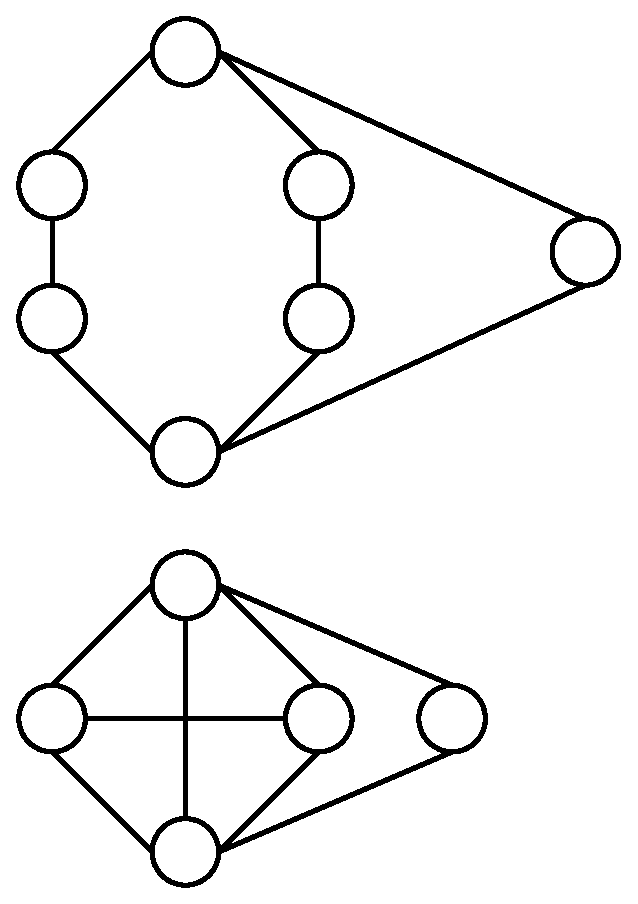
\includegraphics{6.eps}
	\caption{Grafy přátelství pro názornost}
	\label{fig:graphs}
\end{figure}

\end{document}
